%\pdfminorversion=4	
%\pdfobjcompresslevel=0

\documentclass[11pt,onlymath,english]{beamer}

\usepackage{amsmath}
\usepackage{mathcomp}
\usepackage{textcomp}
\usepackage{wasysym, marvosym}

\usepackage{animate}
\usepackage{caption}
\usepackage{subcaption}
\usepackage{multirow}
\usepackage{bigstrut}
\usepackage[compatibility=false]{caption}
\usepackage{listings}
\usepackage{media9}
\usepackage{ragged2e}
\usepackage{textpos}
\usepackage[percent]{overpic}
\usepackage{graphicx}

% Table option
\newcommand{\minitab}[2][l]{\begin{tabular}{#1}#2\end{tabular}}

\makeatletter

% Define the Waterloo theme here
\usetheme{Waterloo}

\usepackage{babel}

\graphicspath{{../figs/}}



%%%%%%%%%%%%%%%%%%%%%%%%%%%%   DOCUMENT BEGINS
\begin{document}


% TITLE PAGE
\title[\emph{Predictive Modelling of Multi-Physics Interaction }]
    {\vspace*{1.1cm}\\Predictive Modelling of Multi-Physics Interaction \vspace*{0.1cm}}
\date{August 9, 2018}
\author{author}
\institute[University of Waterloo]
    {Multi-Physics Interaction Laboratory \\ Mechanical and Mechatronics Engineering\\University of Waterloo}
{
\setbeamertemplate{footline}{} 


% Organize the elements of the title page
\begin{frame}
    \titlepage
    \vspace*{0cm}
    \centering
    \begin{minipage}{0.45\textwidth}
        \vspace*{-0.1cm}
        \includegraphics[width=\linewidth]{identity/universityofwaterloo_black}
    \end{minipage}
\end{frame}
}
\addtocounter{framenumber}{-1}  


% Input each individual section here (add sections as necessary)
%!TEX root = ../MPILAB_template.tex
\graphicspath{{../figs/}}

\section{Simulation challenges in  rockets}


\begin{frame}{Application of AI to combustion}
\begin{itemize}
\item On-going collaboration between Prof Crowley and  Prof Hickey 
\item Improving flamelet pre-tabulation by pre-training an N-dimensional DNN
\item Address dimensionality problems in combustion modelling for complex flows (variable pressure, wall heat transfer, complex thermodynamics etc.)
\end{itemize}
\begin{figure}
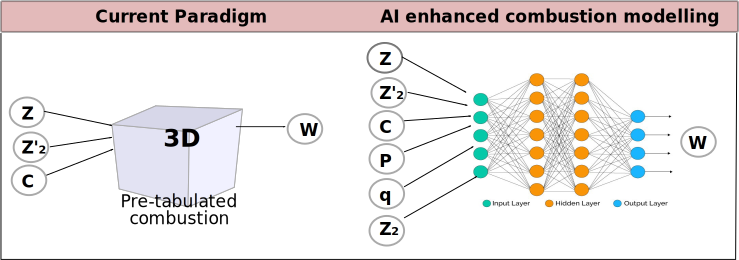
\includegraphics[width=\textwidth]{figs/AI_combustion.png}
\end{figure}
\end{frame}


\section{Concluding Remarks}
\begin{frame}{Conclusion}
\begin{itemize}
\item Multiphysics problems with supercritical flows encountered in many applications: energy production, nuclear engineering (SWCR), automotive engineering (diesel injection systems), aerospace propulsion
\end{itemize}
\end{frame}

\begin{frame}[c]{}
\begin{center}
{\LARGE{Thanks!}}\\
\vspace{0.8cm}

\url{jean-pierre.hickey@uwaterloo.ca}\\
\url{www.mpilab.ca}
\end{center}
\end{frame}





%   BIBLIOGRAPHY
\bibliography{./sections/references}
\bibliographystyle{aiaa}


%%%%%%%%%%%%%%%%%%%%%%%%%%%%   DOCUMENT ENDS
\end{document}
